\documentclass[11pt]{book}
\usepackage{fontspec}
\setmainfont{TeX Gyre Pagella}
\usepackage[margin=1in]{geometry}
\usepackage{xcolor}
\usepackage{tikz}
\usetikzlibrary{arrows.meta,shapes.geometric,shapes.misc}
\usepackage{amssymb}
\usepackage{enumitem}
\usepackage{titlesec}

\titleformat{\chapter}[display]{\bfseries\Large}{Sproll 06}{0.5em}{\Huge}
\titleformat{\section}{\bfseries\large}{\thesection}{0.6em}{}

\newenvironment{algorithmproc}[1]{\vspace{0.6em}\noindent\rule{\linewidth}{0.6pt}\\[0.2em]\textbf{How to Tell: #1}\\[0.3em]}{\\[0.2em]\noindent\rule{\linewidth}{0.6pt}\vspace{0.6em}}
\newenvironment{practicenow}{\vspace{0.6em}\noindent\rule{\linewidth}{0.6pt}\\[0.2em]\textbf{Practice Now}\\[0.3em]}{\\[0.2em]\noindent\rule{\linewidth}{0.6pt}\vspace{0.6em}}
\newenvironment{exercisebox}[1]{\vspace{0.8em}\noindent\rule{\linewidth}{0.6pt}\\[0.2em]\textbf{Exercises: #1}\\[0.3em]\begin{enumerate}[label=\arabic*., itemsep=0.4em]}{\end{enumerate}\noindent\rule{\linewidth}{0.6pt}\vspace{0.6em}}
\newenvironment{trythis}{\vspace{0.6em}\noindent\rule{\linewidth}{0.6pt}\\[0.2em]\textbf{Try This}\\[0.3em]}{\\[0.2em]\noindent\rule{\linewidth}{0.6pt}\vspace{0.6em}}
\newenvironment{summarybox}{\vspace{0.6em}\noindent\rule{\linewidth}{0.6pt}\\[0.2em]\textbf{What We Learned}\\[0.3em]}{\\[0.2em]\noindent\rule{\linewidth}{0.6pt}\vspace{0.6em}}

\begin{document}
\begin{titlepage}
\centering
\vspace*{1.4in}
{\Huge \textbf{SPROLL 06}}\\[0.5in]
{\huge Look Through a Rule}\\[0.8in]
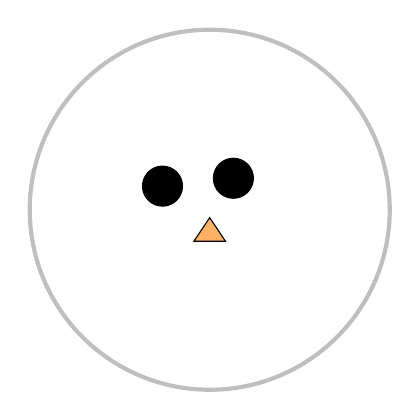
\begin{tikzpicture}
\filldraw[fill=black] (-0.6,0.3) circle (0.1in);
\filldraw[fill=black] (0.3,0.4) circle (0.1in);
\draw[fill=orange!60] (-0.2,-0.4) -- (0,-0.1) -- (0.2,-0.4) -- cycle;
\draw[line width=1.5pt, gray!50] (0,0) circle (0.9in);
\end{tikzpicture}\\[0.8in]
{\Large The Sproll Curriculum}\\[0.2in]
{\large Cycle I: Pops --- Things, Differences, and Counting}
\end{titlepage}

\tableofcontents

\chapter*{Before You Begin}
\addcontentsline{toc}{chapter}{Before You Begin}

Every workbook so far has carefully avoided asking you to calculate anything. This is the workbook where that changes, and it changes for a specific reason. Before you count something, or measure it, or evaluate it, you are always using some rule for what to pay attention to and what to ignore, whether or not you notice you are using one. This workbook makes that rule visible, and introduces the fourth and final primitive action in this curriculum: Collapse.

\chapter{The Same Group, Counted Different Ways}

\section{One Fruit Bowl, Several Honest Answers}

Imagine a fruit bowl containing three apples, two bananas, and one orange. Someone asks, ``how many things are in the bowl?'' A perfectly correct answer is six. Someone else asks, ``how many kinds of fruit are in the bowl?'' A perfectly correct answer is three. A third person asks, ``how many apples are in the bowl?'' The correct answer is three again, but for a completely different reason. All three answers are correct, and all three describe the exact same bowl of fruit.

\begin{center}
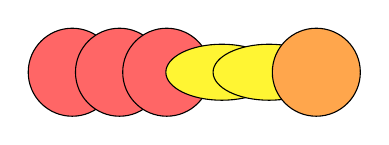
\begin{tikzpicture}
\filldraw[fill=red!60] (-1.2,0.2) circle (0.22in);
\filldraw[fill=red!60] (-0.6,0.2) circle (0.22in);
\filldraw[fill=red!60] (0,0.2) circle (0.22in);
\filldraw[fill=yellow!80] (0.7,0.2) ellipse (0.28in and 0.14in);
\filldraw[fill=yellow!80] (1.3,0.2) ellipse (0.28in and 0.14in);
\filldraw[fill=orange!70] (1.9,0.2) circle (0.22in);
\end{tikzpicture}
\end{center}

Nothing about the bowl changed between the three questions. What changed each time was the rule being used to look at it: count every piece of fruit, count the kinds of fruit, or count only one specific kind. This curriculum has a name for applying a rule like this to something already constructed: a \textbf{Collapse}. To collapse a group under a rule means to look at it through that rule and see what comes out, a number, a description, a smaller group, whatever the rule produces.

\begin{algorithmproc}{Reading a Collapse}
Whenever you are given a count, a description, or a summary of something, ask what rule produced it. The same underlying thing can honestly produce very different summaries, and neither summary is more real than the other; each is simply the result of collapsing the same thing under a different rule.
\end{algorithmproc}

\begin{practicenow}
Look at a shelf, a drawer, or a small collection of objects near you. Count it under at least two different rules (for example: total objects, versus objects of one particular color or type). Confirm that you get two different, equally correct numbers.
\end{practicenow}

\begin{exercisebox}{Section 1.1}
\item Using the fruit bowl example, explain why ``six'' and ``three'' can both be correct answers to the question ``how many are there,'' without either one being wrong.
\item Describe a real collection of objects in your life that could honestly be counted in at least three different ways, and give the rule for each way.
\item Challenge: is it possible for a rule to be so strict that it counts zero things in a group that clearly has objects in it? Give an example.
\end{exercisebox}

\chapter{A Rule Applied to a Record}

\section{Counting a History, Not Just a Picture}

This same idea applies directly to the histories this curriculum has been building since Sproll 01. Recall a ledger recording several Pops and a Refuse. Under one rule, you might count every entry in the ledger, Pops and Refuses together. Under a different rule, you might count only the Pops, ignoring anything that was refused. Both are legitimate ways to collapse the same ledger; they simply answer different questions about it.

\begin{algorithmproc}{Choosing a Rule}
Before counting or summarizing a record, decide explicitly what you want the count to represent: every event, only certain kinds of events, or something else entirely. State the rule before you start counting, so that your answer can be checked against the rule you actually used.
\end{algorithmproc}

\begin{trythis}
Write out a short made-up record of five events, a mix of choices and refusals. Count it once under the rule ``count everything'' and again under the rule ``count only the choices.'' Confirm the two counts are different.
\end{trythis}

\begin{exercisebox}{Section 2.1}
\item A class has 20 students, 12 of whom are wearing sneakers. Under the rule ``count every student,'' the answer is 20. Under the rule ``count only students wearing sneakers,'' the answer is 12. Invent a third rule for the same class and give its answer.
\item Explain why it does not make sense to ask ``what is the real count'' of something without first asking ``real count under which rule.''
\item Challenge: can two completely different rules ever produce the exact same number, purely by coincidence, for the same group? Try to construct an example.
\end{exercisebox}

\chapter{Make Your Own Rule}

\section{Collapse Is Something You Choose}

The most important habit this workbook can leave you with is this: a rule for looking at something is not handed down from nowhere. Someone chooses it, usually because it answers a question they actually care about. Ordinary counting and ordinary arithmetic, the kind you have likely already learned or are learning elsewhere, are themselves specific, very useful choices of rule, not the one and only correct way to look at a group of things.

\begin{trythis}
Invent your own counting rule for a group of mixed objects (a pile of coins, a box of crayons, a bag of mixed candy). State your rule clearly, apply it, and then invent a second rule that gives a different answer for the exact same pile.
\end{trythis}

\begin{summarybox}
A Collapse applies a chosen rule to something already constructed and produces a result: a count, a description, a smaller group. The same underlying thing can honestly produce different, equally correct results under different rules. Ordinary counting and arithmetic are themselves specific choices of rule, not the only possible way to look at a group.
\end{summarybox}

\begin{exercisebox}{Section 3.1}
\item Explain, in your own words, why this workbook says ``a rule is chosen'' rather than ``a rule is discovered.''
\item Pick any group of objects around you right now and produce three different, correct counts of it under three different rules.
\item Challenge: can you think of a situation where choosing the wrong rule for a count could actually cause a real problem (not just a different number, but a bad decision based on it)?
\end{exercisebox}

\chapter*{Looking Ahead}
\addcontentsline{toc}{chapter}{Looking Ahead}

Sproll 00 and Sproll 02 both left a question open: whether two things that look alike, or two histories that reach the same picture, are really ``the same.'' Now that you have Collapse and a chosen rule available, both questions can finally be answered properly. That is the subject of the next workbook, Sproll 07: Same Picture, Different Story.

\chapter*{For Parents and Teachers}
\addcontentsline{toc}{chapter}{For Parents and Teachers}

This workbook introduces Collapse, the fourth and final primitive action this curriculum is built from, and is the first workbook in the series in which any calculation occurs, consistent with this curriculum's house style, which withholds calculation until a rule-relative notion of observation has been established. Ordinary arithmetic evaluation is deliberately framed here as one specific, useful Collapse rule among many possible rules, rather than as a privileged or default operation, since a central later idea in this curriculum (that equality and identity are always relative to a stated rule) depends on this framing being in place first.

\end{document}
